\documentclass[12pt, titlepage]{article}

\usepackage{fullpage}
\usepackage[round]{natbib}
\usepackage{multirow}
\usepackage{booktabs}
\usepackage{tabularx}
\usepackage{graphicx}
\usepackage{float}
\usepackage{hyperref}

\usepackage{indentfirst}
\usepackage{enumerate}
\usepackage[shortlabels]{enumitem}
\usepackage{xcolor}
\usepackage{ulem}

\hypersetup{
colorlinks,
citecolor=blue,
filecolor=black,
linkcolor=red,
urlcolor=blue
}

%% Comments

\usepackage{color}

\newif\ifcomments\commentstrue %displays comments
%\newif\ifcomments\commentsfalse %so that comments do not display

\ifcomments
\newcommand{\authornote}[3]{\textcolor{#1}{[#3 ---#2]}}
\newcommand{\todo}[1]{\textcolor{red}{[TODO: #1]}}
\else
\newcommand{\authornote}[3]{}
\newcommand{\todo}[1]{}
\fi

\newcommand{\wss}[1]{\authornote{blue}{SS}{#1}} 
\newcommand{\plt}[1]{\authornote{magenta}{TPLT}{#1}} %For explanation of the template
\newcommand{\an}[1]{\authornote{cyan}{Author}{#1}}

%% Common Parts

\newcommand{\progname}{REVITALIZE} % PUT YOUR PROGRAM NAME HERE
\newcommand{\authname}{Team 13, REVITALIZE
\\ Bill Nguyen
\\ Syed Bokhari
\\ Hasan Kibria
\\ Youssef Dahab
\\ Logan Brown
\\ Mahmoud Anklis} % AUTHOR NAMES                  

\usepackage{hyperref}
    \hypersetup{colorlinks=true, linkcolor=blue, citecolor=blue, filecolor=blue,
                urlcolor=blue, unicode=false}
    \urlstyle{same}
                                


\newcounter{acnum}
\newcommand{\actheacnum}{AC\theacnum}
\newcommand{\acref}[1]{AC\ref{#1}}

\newcounter{ucnum}
\newcommand{\uctheucnum}{UC\theucnum}
\newcommand{\uref}[1]{UC\ref{#1}}

\newcounter{mnum}
\newcommand{\mthemnum}{M\themnum}
\newcommand{\mref}[1]{M\ref{#1}}

\begin{document}

\title{Module Guide for \progname{}} 
\author{\authname}
\date{\today}

\maketitle

\pagenumbering{roman}

\section{Revision History}

\begin{tabularx}{\textwidth}{p{3cm}p{2cm}X}
	\toprule {\bf Date} & {\bf Version} & {\bf Notes}\\
	\midrule
	January 17th, 2023 & Bill Nguyen  & Added MG for Main Menu and Calendar\\
	January 18th, 2023 & Youssef Dahab & Added Intro, MG for Login, Container, Label, \& Circular Slider\\
	January 18th, 2023 & Hasan Kibria & Added to SRS Connection, Module Decomposition\\	
	January 18th, 2023 & Syed Bokhari & Matrix Traceability with FR\\	
	January 18th, 2023 & Bill Nguyen  & Added Module Decomposition and Uses Hierarchy\\
	January 18th, 2023 & Logan Brown  & Added Anticipated Changes\\
	January 18th, 2023 & Mahmoud Anklis  & Added Unlikely Changes\\
\bottomrule
\end{tabularx}

\newpage

\section{Reference Material}

This section records information for easy reference.

\subsection{Abbreviations and Acronyms}

\renewcommand{\arraystretch}{1.2}
\begin{tabular}{l l} 
	\toprule		
	\textbf{symbol} & \textbf{description}\\
	\midrule 
	AC & Anticipated Change\\
	DAG & Directed Acyclic Graph \\
	M & Module \\
	MG & Module Guide \\
	OS & Operating System \\
	R & Requirement\\
	SC & Scientific Computing \\
	SRS & Software Requirements Specification\\
	\progname & Explanation of program name\\
	UC & Unlikely Change \\
	%\wss{etc.} & \wss{...}\\
	\bottomrule
\end{tabular}\\

\newpage

\tableofcontents

\listoftables

\listoffigures

\newpage

\pagenumbering{arabic}

\section{Introduction}
REVITALIZE is an app designed to supply users with the means to improve their health by providing them with meal recipe's based on their nutritional preferences, a personalized workouts planner and a sleep tracker.  

\subsection{Purpose}
The purpose of this document is to outline REVITALIZE's modular structure using decomposition based on the principle of information hiding to allow project members to easily identify parts within the app \citep{Parnas1972a}.

\subsection{Scope}
This document outlines the modules which are based off the requirements specified
in the \href{https://github.com/BillNguyen1999/REVITALIZE/blob/main/docs/SRS/SRS.pdf}{\textbf{Software Requirements Specification}}. In addition, the external behavior of those modules is specified in the \href{https://github.com/BillNguyen1999/REVITALIZE/blob/main/docs/Design/SoftDetailedDes/MIS.pdf}{\textbf{Module Interface Specification}}.

\subsection{MG Overiew}
\begin{itemize}
	\item Section \ref{SecChange} lists the anticipated and unlikely changes of the software requirements. 
	\item Section \ref{SecMH} summarizes the module decomposition that was constructed according to the likely changes. 
	\item Section \ref{SecConnection} specifies the connection between the software requirements and the modules. \item Section \ref{SecMD} is a description of the modules. 
	\item Section \ref{SecTM} includes two traceability matrices. One checks the completeness of the design against the requirements provided in the SRS. The other shows the relation between anticipated changes and the modules. 
	\item Section \ref{SecUse} describes the use hierarchy between modules. 
\end{itemize}

\section{Anticipated and Unlikely Changes} \label{SecChange}

This section lists possible changes to the system. According to the likeliness
of the change, the possible changes are classified into two
categories. Anticipated changes are listed in Section \ref{SecAchange}, and
unlikely changes are listed in Section \ref{SecUchange}.

\subsection{Anticipated Changes} \label{SecAchange}

Anticipated changes are the source of the information that is to be hidden
inside the modules. Ideally, changing one of the anticipated changes will only
require changing the one module that hides the associated decision. The approach
adapted here is called design for
change.

\begin{description}
	\item[\refstepcounter{acnum} \actheacnum \label{ac1}:] The format the date is stored in
	\item[\refstepcounter{acnum} \actheacnum \label{ac2}:] The labels of buttons to navigate screens
	\item[\refstepcounter{acnum} \actheacnum \label{ac3}:] Colouring of screens
	\item[\refstepcounter{acnum} \actheacnum \label{ac4}:] Input text box length and location
	\item[\refstepcounter{acnum} \actheacnum \label{ac5}:] Layout of calendar
	\item[\refstepcounter{acnum} \actheacnum \label{ac6}:] Nutrition display format
	\item[\refstepcounter{acnum} \actheacnum \label{ac7}:] Recipe search criteria
	\item[\refstepcounter{acnum} \actheacnum \label{ac8}:] Recipe query result format
	\item[\refstepcounter{acnum} \actheacnum \label{ac9}:] Custom meal input format
	\item[\refstepcounter{acnum} \actheacnum \label{ac10}:] Workout display format
	\item[\refstepcounter{acnum} \actheacnum \label{ac11}:] Exercise list search criteria
	\item[\refstepcounter{acnum} \actheacnum \label{ac12}:] Exercise query result format
	\item[\refstepcounter{acnum} \actheacnum \label{ac13}:] Sleep time input (sensitivity of circular scroll bar)
\end{description}

\subsection{Unlikely Changes} \label{SecUchange}

The module design should be as general as possible. However, a general system is
more complex. Sometimes this complexity is not necessary. Fixing some design
decisions at the system architecture stage can simplify the software design. If
these decision should later need to be changed, then many parts of the design
will potentially need to be modified. Hence, it is not intended that these
decisions will be changed.

\begin{description}
	\item[\refstepcounter{ucnum} \uctheucnum \label{ucIO}:] Input/Output devices
	(Input: File and/or Keyboard, Output: File, Memory, and/or Screen)
	\item[\refstepcounter{ucnum} \uctheucnum \label{uc2}:] The Android operating system
	\item[\refstepcounter{ucnum} \uctheucnum \label{uc3}:] The calls to the Meal API to search for recipes based on nutritional input
	\item[\refstepcounter{ucnum} \uctheucnum \label{uc4}:] The database to store user information
	\item[\refstepcounter{ucnum} \uctheucnum \label{uc5}:] The selection of different exercises
\end{description}

\section{Module Hierarchy} \label{SecMH}

This section provides an overview of the module design. Modules are summarized
in a hierarchy decomposed by secrets in Table \ref{TblMH}. The modules listed
below, which are leaves in the hierarchy tree, are the modules that will
actually be implemented.

\begin{description}
	\item [\refstepcounter{mnum} \mthemnum \label{m1}:] Main Menu
	\item [\refstepcounter{mnum} \mthemnum \label{m2}:] Calendar
	\item [\refstepcounter{mnum} \mthemnum \label{m3}:] Login
	\item [\refstepcounter{mnum} \mthemnum \label{m4}:] Container
	\item [\refstepcounter{mnum} \mthemnum \label{m5}:] Label
	\item [\refstepcounter{mnum} \mthemnum \label{m6}:] Circular Slider
	\item [\refstepcounter{mnum} \mthemnum \label{m7}:] Diet Log
	\item [\refstepcounter{mnum} \mthemnum \label{m8}:] Search or Add Food
	\item [\refstepcounter{mnum} \mthemnum \label{m9}:] Custom Meal
	\item [\refstepcounter{mnum} \mthemnum \label{m10}:] Search Recipe
	\item [\refstepcounter{mnum} \mthemnum \label{m11}:] Recipe Results
	\item [\refstepcounter{mnum} \mthemnum \label{m12}:] Recipe Details
	\item [\refstepcounter{mnum} \mthemnum \label{m13}:] FoodT
	\item [\refstepcounter{mnum} \mthemnum \label{m14}:] Workout Display
	\item [\refstepcounter{mnum} \mthemnum \label{m15}:] Workout Edit
	\item [\refstepcounter{mnum} \mthemnum \label{m16}:] Workout Log
	\item [\refstepcounter{mnum} \mthemnum \label{m17}:] ExerciseT
	\item [\refstepcounter{mnum} \mthemnum \label{m18}:] Signup
\end{description}


\begin{table}[h!]
	\centering
	\begin{tabular}{p{0.3\textwidth} p{0.6\textwidth}}
		\toprule
		\textbf{Level 1} & \textbf{Level 2}\\
		\midrule
		
		{Hardware-Hiding Module} & ~ \\
		\midrule
		
		\multirow{7}{0.3\textwidth}{Behaviour-Hiding Module} & Main Menu\\
		& Calendar\\
		& Login\\
		& Container\\
		& Label\\
		& Circular Slider\\
		& Diet Log\\ 
		& Search or Add Food\\
		& Custom Meal\\
		& Search Recipe\\
		& Recipe Results\\
		& Recipe Details\\
		& Workout Display\\
		& Workout Edit\\
		& Workout Log\\
		& Signup\\
		\midrule
		
		\multirow{3}{0.3\textwidth}{Software Decision Module} & FoodT\\
		& ExerciseT\\
		\bottomrule
		
	\end{tabular}
	\caption{Module Hierarchy}
	\label{TblMH}
\end{table}

\section{Connection Between Requirements and Design} \label{SecConnection}

The system design of REVITALIZE is founded upon the requirements previously set in the SRS. It is designed to cater for every single requirement attributed to this project. Hence, the design is decomposed into modular pieces of functionality which each help serve the fulfillment of aforementioned requirements. Specifications on how each module relates to (a) requirement(s) can be found in Section \textcolor{red}{\sout{8}} \textcolor{red}{\ref{SecTM}}.\\
The functional outlook of each module can be understood by its name and, if needed, its access programs detailed in the MIS. After realizing the functionality of each module, the connections outlined in the Traceability Matrix in Section \textcolor{red}{\sout{8}} \textcolor{red}{\ref{SecTM}} should be clear and easily comprehended.
\section{Module Decomposition} \label{SecMD}

Modules are decomposed according to the principle of ``information hiding''
proposed by \citet{ParnasEtAl1984}. The \emph{Secrets} field in a module
decomposition is a brief statement of the design decision hidden by the
module. The \emph{Services} field specifies \emph{what} the module will do
without documenting \emph{how} to do it. For each module, a suggestion for the
implementing software is given under the \emph{Implemented By} title. If the
entry is \emph{OS}, this means that the module is provided by the operating
system or by standard programming language libraries.  \emph{\progname{}} means the
module will be implemented by the \progname{} software.

Only the leaf modules in the hierarchy have to be implemented. If a dash
(\emph{--}) is shown, this means that the module is not a leaf and will not have
to be implemented.

\subsection{Hardware Hiding Modules }
N/A

\subsection{Behaviour-Hiding Module}

\subsubsection{Main Menu (\mref{m1})}
\begin{description}
	\item[Secrets:]\textcolor{red}{\sout{Method to visualize main menu}}\textcolor{red}{. The interface of REVITALIZE that the user interacts with after logging in}
	\item[Services:]Visualizes main menu by displaying interactive buttons to navigate to Diet, Exercise and/or Sleep section. Also shows current date in the top-center of screen which is clickable to display calendar screen. Finally a backward and forward button to display previous and next day.
	\item[Implemented By:] REVITALIZE
\end{description}

\subsubsection{Calendar (\mref{m2})}
\begin{description}
	\item[Secrets:]\textcolor{red}{\sout{Method to visualize calendar screen}}\textcolor{red}{. The user interface that displays the calendar to the user}
	\item[Services:]Visualizes calendar by displaying interactive screen that shows current month and the respective days of the month, where user can click on desired day. Also has a backward and forward button to display previous and next month.
	\item[Implemented By:] REVITALIZE
\end{description}

\subsubsection{Login (\mref{m3})}
\begin{description}
	\item[Secrets:]\textcolor{red}{\sout{Method to visualize login screen}}\textcolor{red}{. The interface of REVITALIZE that the user interacts with once the app is launched}
	\item[Services:]Visualizes login screen by displaying interactive screen that shows name or email and password input text boxes for user to enter. Also has a login button for user to login. Moreover, has forgot password and sign up links for user to reset password or sign up respectively.
	\item[Implemented By:] REVITALIZE
\end{description}

\subsubsection{Container (\mref{m4})}
\begin{description}
	\item[Secrets:]\textcolor{red}{\sout{Method to visualize sleep screen}}\textcolor{red}{. The user interface that the user interacts with when viewing the sleep screen}
	\item[Services:]Visualizes sleep screen by displaying interactive screen that shows labels and circular slider in sleep screen.
	\item[Implemented By:] REVITALIZE
\end{description}

\subsubsection{Label (\mref{m5})}
\begin{description}
	\item[Secrets:]\textcolor{red}{\sout{Method to visualize certain components in sleep screen}}\textcolor{red}{. The component that displays the bed and ring icon images on screen}
	\item[Services:]Visualizes bed icon, \textcolor{red}{\sout{"}}\textcolor{red}{``}BEDTIME" text, ring icon, \textcolor{red}{\sout{"}}\textcolor{red}{``}WAKE UP" text, user set bed-time and wake-up time in sleep screen.
	\item[Implemented By:] REVITALIZE
\end{description}

\subsubsection{Circular Slider (\mref{m6})}
\begin{description}
	\item[Secrets:]\textcolor{red}{\sout{Method to visualize circular slider and total sleep time in sleep screen}}\textcolor{red}{. The circular slider user interface component that the user interacts with when viewing the sleep screen to set bed and wake up times.}
	\item[Services:]Visualizes circular slider by displaying interactive screen that shows circular slider that user can slide to set bed-time and wake-up times. Also shows user their total sleep time.
	\item[Implemented By:] REVITALIZE
\end{description}

\subsubsection{Diet Log Module (\mref{m7})}
\begin{description}
	\item[Secrets:]\textcolor{red}{\sout{Method to visualize daily diet log screen}}\textcolor{red}{. The user interface screen that displays to the user their food log with information regarding their calories, proteins, fat, and carbs}
	\item[Services:]Visualizes diet log by displaying interactive table with adherent food entries. Also shows net nutritional intake for the day.
	\item[Implemented By:] REVITALIZE
\end{description}

\subsubsection{Search or Add Food Module (\mref{m8})}
\begin{description}
	\item[Secrets:]\textcolor{red}{\sout{Method to visualize decision making screen between adding a custom food and searching an online recipe}}\textcolor{red}{. The user interface screen that allows the user to search an online recipe or add a custom meal}
	\item[Services:]Visualizes decision making screen by displaying two buttons, each representative of the possible decision made, which leads to another screen to help user complete their preferred decision.
	\item[Implemented By:] REVITALIZE
\end{description}

\subsubsection{Custom Meal Module (\mref{m9})}
\begin{description}
	\item[Secrets:]\textcolor{red}{\sout{Method to visualize custom meal logger}}\textcolor{red}{. The user interface screen that allows the user to add a custom meal after inputting their meal name, calories, protein, carbohydrates, and fats}
	\item[Services:]Visualizes custom meal logger by displaying input fields which take information relative to custom meal.
	\item[Implemented By:] REVITALIZE
\end{description}

\subsubsection{Search Recipe Module (\mref{m10})}
\begin{description}
	\item[Secrets:]\textcolor{red}{\sout{Method to visualize app-internal search engine for recipes with custom filterization}}\textcolor{red}{. The user interface screen that allows the user to search an online recipe after entering their meal name, calories, and protein type}
	\item[Services:]Visualizes app-internal search engine for recipes by displaying multiple filtering inputs and a search button which retrieves filtered recipe data.
	\item[Implemented By:] REVITALIZE
\end{description}

\subsubsection{Recipe Results Module (\mref{m11})}
\begin{description}
	\item[Secrets:]\textcolor{red}{\sout{Method to visualize search results from search query produced through Search Recipe Module}}\textcolor{red}{. The user interface screen that displays to the user a list of recipe results after searching for a meal's recipe}
	\item[Services:]Visualizes search results by displaying a list of scrollable search results with a small description for each result.
	\item[Implemented By:] REVITALIZE
\end{description}

\subsubsection{Recipe Details Module (\mref{m12})}
\begin{description}
	\item[Secrets:]\textcolor{red}{\sout{Method to visualize detailed information about each recipe}}\textcolor{red}{. The user interface screen that displays to the user the recipe ingredients along with its calories, proteins, carbs, and fats}
	\item[Services:]Visualizes detailed information about each recipe using a paragraph description and an image
	\item[Implemented By:] REVITALIZE
\end{description}

\subsubsection{Workout Display Module (\mref{m14})}
\begin{description}
	\item[Secrets:]\textcolor{red}{\sout{Method to visualize the workout of the day}}\textcolor{red}{. The user interface screen that displays to the user their workouts with details such as workout name, reps, sets, and weights}
	\item[Services:]Visualizes workout screen by displaying the workout on the given date. Also provides 'add workout' button to navigate to the Workout Edit module.
	\item[Implemented By:] REVITALIZE
\end{description}

\subsubsection{Workout Edit Module (\mref{m15})}
\begin{description}
	\item[Secrets:]\textcolor{red}{\sout{Method to visualize changes made to the workout of the day}}\textcolor{red}{. The user interface screen that allows the user to edit their workout information such as workout name, sets, reps, and weights}
	\item[Services:]Allows addition and removal of exercises to the workout on the selected date. Provides 'add exercise' and 'save' button to add a new exercise and save changes respectively.
	\item[Implemented By:] REVITALIZE
\end{description}

\subsubsection{Workout Log Module (\mref{m16})}
\begin{description}
	\item[Secrets:]\textcolor{red}{\sout{Method to store contents of workouts}}\textcolor{red}{. The user interface screen that displays to users their past and present workouts}
	\item[Services:]Provides structure to store workouts. Provides access to past workouts.
	\item[Implemented By:] REVITALIZE
\end{description}

\subsubsection{Signup Module (\mref{m18})}
\begin{description}
	\item[Secrets:]\textcolor{red}{\sout{Method to visualize signup screen}}\textcolor{red}{. The user interface screen that the user uses to create an account with REVITALIZE} 
	\item[Services:]Provides input text boxes for user to create an account. Also has a signup button and back to login page button to create an account or navigate back to the login page respectively.
	\item[Implemented By:] REVITALIZE
\end{description}


\subsection{Software Decision Module}

\subsubsection{FoodT Module (\mref{m13})}
\begin{description}
	\item[Secrets:] Data structure to hold information about each distinct food
	\item[Services:] \textcolor{red}{None}
	\item[Implemented By:] REVITALIZE
\end{description}

\subsubsection{ExerciseT Module (\mref{m17})}
\begin{description}
	\item[Secrets:]Data structure to describe information of a specific exercise
	\item[Services:] \textcolor{red}{None}
	\item[Implemented By:] REVITALIZE
\end{description}

\section{Traceability Matrix} \label{SecTM}

This section shows two traceability matrices: between the modules and the
requirements and between the modules and the anticipated changes.

% the table should use mref, the requirements should be named, use something
% like fref
\begin{table}[H]
	\centering
	\begin{tabular}{p{0.2\textwidth} p{0.6\textwidth}}
		\toprule
		\textbf{Req.} & \textbf{Modules}\\
		\midrule
		FR1 & \mref{m3}\\
		FR2 & \mref{m3}\\
		FR3 & \mref{m3}\\
		FR4 & \textcolor{red}{\sout{\mref{m3}}}\textcolor{red}{. \mref{m18}}\\
		FR5 & \mref{m3}\\
		FR6 & \mref{m3}\\
		FR7 & \mref{m3}\\
		FR8 & \textcolor{red}{\sout{\mref{m3}}}\textcolor{red}{. \mref{m18}}\\
		FR9 & \textcolor{red}{\sout{\mref{m3}}}\textcolor{red}{. \mref{m18}}\\
		FR10 & \textcolor{red}{\sout{\mref{m3}}}\textcolor{red}{. \mref{m18}}\\
		FR11 & \textcolor{red}{\sout{\mref{m3}}}\textcolor{red}{. \mref{m18}}\\
		FR12 & \textcolor{red}{\sout{\mref{m18}}}\textcolor{red}{. \mref{m7}}\\
		FR13 & \textcolor{red}{\sout{\mref{m18}}}\textcolor{red}{. \mref{m7}}\\
		FR14 & \textcolor{red}{\sout{\mref{m18}}}\textcolor{red}{. \mref{m7}}\\
		FR15 & \textcolor{red}{\sout{\mref{m1}}}\textcolor{red}{. \mref{m8}}\\
		FR16 & \textcolor{red}{\sout{\mref{m1}}}\textcolor{red}{. \mref{m10}}\\
		FR17 & \textcolor{red}{\sout{\mref{m1}}}\textcolor{red}{. \mref{m11}}\\
		FR18 & \textcolor{red}{\sout{\mref{m1}}}\textcolor{red}{. \mref{m11}}\\
		FR19 & \textcolor{red}{\sout{\mref{m7}}}\textcolor{red}{. \mref{m9}}\\
		FR20 & \textcolor{red}{\sout{\mref{m7}}}\textcolor{red}{. \mref{m10}, \mref{m11}}\\
		FR21 & \textcolor{red}{\sout{\mref{m7}}}\textcolor{red}{. \mref{m14}}\\
		FR22 & \textcolor{red}{\sout{\mref{m8}}}\textcolor{red}{. \mref{m14}}\\
		FR23 & \textcolor{red}{\sout{\mref{m8}}}\textcolor{red}{. \mref{m15}}\\
		FR24 & \mref{m8}, \mref{m10}\\
		FR25 & \textcolor{red}{\sout{\mref{m10}}}\textcolor{red}{. \mref{m5}}\\
		FR26 & \textcolor{red}{\sout{\mref{m11}}}\textcolor{red}{. \mref{m14}}\\
		FR27 & \mref{m11}\\
		FR28 & \mref{m9}\\
		\textcolor{red}{\sout{FR29}} & \textcolor{red}{\sout{\mref{m9}}}\\
		\textcolor{red}{\sout{FR30}} & \textcolor{red}{\sout{\mref{m1},}} \textcolor{red}{\sout{\mref{m4},}} \textcolor{red}{\sout{\mref{m7},}} \textcolor{red}{\sout{\mref{m14}}}\\
		\textcolor{red}{\sout{FR31}} & \textcolor{red}{\sout{\mref{m14}}}\\
		\textcolor{red}{\sout{FR32}} & \textcolor{red}{\sout{\mref{m14}}}\\
		\textcolor{red}{\sout{FR33}} & \textcolor{red}{\sout{\mref{m15}}}\\
		\textcolor{red}{\sout{FR34}} & \textcolor{red}{\sout{\mref{m15}}}\\
		\textcolor{red}{\sout{FR35}} & \textcolor{red}{\sout{\mref{m17}}}\\
		\textcolor{red}{\sout{FR36}} & \textcolor{red}{\sout{\mref{m5}}}\\
		\textcolor{red}{\sout{FR37}} & \textcolor{red}{\sout{\mref{m6}}}\\
		\bottomrule
	\end{tabular}
	\caption{Trace Between Requirements and Modules}
	\label{TblRT}
\end{table}

\begin{table}[H]
	\centering
	\begin{tabular}{p{0.2\textwidth} p{0.6\textwidth}}
		\toprule
		\textbf{AC} & \textbf{Modules}\\
		\midrule
		\acref{ac1} & \mref{m1}\\
		\acref{ac2} & \mref{m1}, \mref{m4}, \mref{m7}, \mref{m14}\\
		\acref{ac3} & \mref{m1}\\
		\acref{ac4} & \mref{m1}\\
		\acref{ac6} & \mref{m7}\\
		\acref{ac7} & \mref{m10}\\
		\acref{ac8} & \mref{m11}\\
		\acref{ac9} & \mref{m9}\\
		\acref{ac10} & \mref{m14}\\
		\acref{ac11} & \mref{m14}\\
		\acref{ac12} & \mref{m14}\\
		\acref{ac13} & \mref{m6}\\
		\bottomrule
	\end{tabular}
	\caption{Trace Between Anticipated Changes and Modules}
	\label{TblACT}
\end{table}

\section{Use Hierarchy Between Modules} \label{SecUse}

In this section, the uses hierarchy between modules is
provided. \citet{Parnas1978} said of two programs A and B that A {\em uses} B if
correct execution of B may be necessary for A to complete the task described in
its specification. That is, A {\em uses} B if there exist situations in which
the correct functioning of A depends upon the availability of a correct
implementation of B.  Figure \ref{FigUH} illustrates the use relation between
the modules. It can be seen that the graph is a directed acyclic graph
(DAG). Each level of the hierarchy offers a testable and usable subset of the
system, and modules in the higher level of the hierarchy are essentially simpler
because they use modules from the lower levels.

\begin{figure}[H]
	\centering
	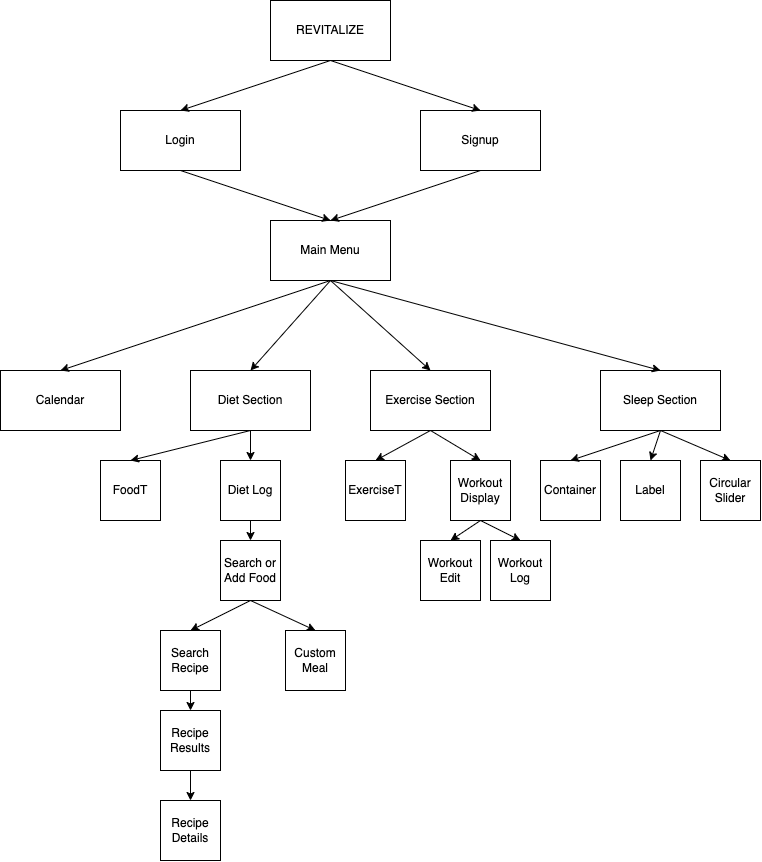
\includegraphics[width=0.7\textwidth]{images/MGDAG.png}
	\caption{Use hierarchy among modules for REVITALIZE}
	\label{FigUH}
\end{figure}

%\section*{References}

\bibliographystyle {plainnat}
\bibliography{../../../refs/References}

\newpage{}

\end{document}